\chapter{Numerical Methods}
\label{chap:chapter-3}
	
Simulating compact binary coalescence requires Einstein's full theory of general relativity.
We approach the problem of evolving black hole-neutron star inspirals and mergers with the Spectral Einstein Code
\footnote{\url{https://black-holes.org/SpEC.html}}
(\SpEC).  
\SpEC uses a two-grid method to simultaneously evolve Einstein's equations~\cite{Lindblom:2007,Szilagyi:2014fna} and the fluid equations~\cite{Duez:2008rb,Foucart:2013a}.
We evolve Einstein's equations using multi-domain pseudospectral methods on what we'll refer to as the GR grid.
For the fluid matter, we evolve the fluid equations on a multi-domain finite volume grid, occasionally referred to in this work as the fluid grid.

In Section \ref{sec:gr-grid}, we discuss the design implementation we use to evolve Einstein's equations with pseudospectral methods in \SpEC.  The finite difference scheme used to evolve the fluid equations is discussed in Section \ref{sec:fd-grid}.  The grid-to-grid communication and time stepping procedure is discussed in Section \ref{sec:communication}.  The implementation of our new mesh refinement algorithm for evolving the FD grid will be discussed in Section \ref{sec:hydro-amr}.  We discuss the necessary refinements to the grids in Section \ref{sec:epochs}.

\section{GR Grid}
\label{sec:gr-grid}

In the 3+1 formalism, three dimensional spatial subsurfaces of four dimensional spacetime are foliated from time, implementing a coordinate system $\{t, x^k\}$.  The line element of the metric is written as
\begin{equation}
ds^2 = g_{ab} {dx}^a {dx}^b = -\alpha^2 {dt}^2 + \gamma_{ij} (dx^i + \beta^i dt) (dx^j + \beta^j dt)
\end{equation} 
defining the lapse $\alpha$, the shift vector $\beta^k$ and the 3-metric $\gamma_{ij}$. 
In \SpEC, we use the generalized harmonic formulation of Einstein's field equations.  By harmonic, we assume the coordinates $x^\alpha$ obey the inhomogeneous  wave equation
\begin{equation}
g_{ab} \nabla^c \nabla_c x^b = H_a (x, g_{ab})
\end{equation}
for some specified harmonic gauge function $H_a$.  Here, we note that $\nabla_c$ is the covariant derivative associated with $g_{ab}$.  


In order to turn the second order time derivatives of Einstein's equations into a set of first order symmetric hyperbolic equations in time, we introduce the following variables:
\begin{align}
\Phi_{iab} &\equiv \partial_i g_{ab} \\
\Pi_{ab} &\equiv n^c \partial_c g_{ab},
\end{align}
the spatial and time derivatives of the metric, respectively, where we have introduced the slice normal $n^c$.  
Therefore, assuming the constraints
\begin{align}
{\cal{C}}_a &\equiv H_a (x, g_{ab} )  \\
{\cal{C}}_{iab} &\equiv \partial_i g_{ab} - \Phi_{iab} 
\end{align}
aren't violated, Einstein's equations can be rewritten in general harmonic form:
\begin{align}
\partial_t g_{ab} &\simeq \beta^k \partial_k g_{ab} \\
\partial_t \Pi_{ab} &\simeq \beta^k \partial_k \Pi_{ab} - \alpha g^{ki} \partial_k \Phi_{iab} \\
\partial_t \Phi_{iab} &\simeq \beta^k \partial_k \Phi_{iab} - \alpha  \partial_i \Pi_{ab}
\end{align}
where we have included only the principal (`$\simeq$') parts to be evolved.  We note that these equations are in symmetric hyperbolic form:
\begin{equation}
\partial_t u^\alpha + {A^{k\alpha}}_\beta \partial_k u^\beta \simeq 0
\end{equation}
The gauge function $H_a$ is chosen given assumptions of the coordinate system dynamics.  
A gauge of $H_a = 0$ is some the ``harmonic'' gauge; 
if $H_a$ is set to some constant other than zero--known as the ``frozen gauge'', it will just advect with the evolution;
during the merger, we generally roll-on a `damped-harmonic'' gauge because the spacetime is so dynamical in black hole-neutron star mergers.

The GR grid is first divided into touching but not overlapping subdomains consisting of: cubed spheres, wedges, and spherical shells (see Figure \ref{fig:pseudospectral-grid}).
The choice of the geometry of the subdomains are chosen so as to reflect the configuration symmetry.  
A penalty method is employed at subdomain interfaces~\cite{Hesthaven1999,Hesthaven2000,Gottlieb2001,Hesthaven1997}.  
In corotating coordinates, the black hole is spherically excised such that the excision surface lies between the inner and outer apparent horizons of the (Kerr) black hole. 
We control the size of the horizon with a function $f(r)$ and the shape of the excision surface as a series of spherical harmonics: $r \rightarrow r + f(r) \sum_{lm} { c_{lm} Y_{lm}(\theta, \varphi) }$, where $r$ is the distance from the coordinate center of the black hole.
The control system also maintains the black hole to be centered on a stationary point, which is done by translational mapping.  

\begin{figure}
	\centering
	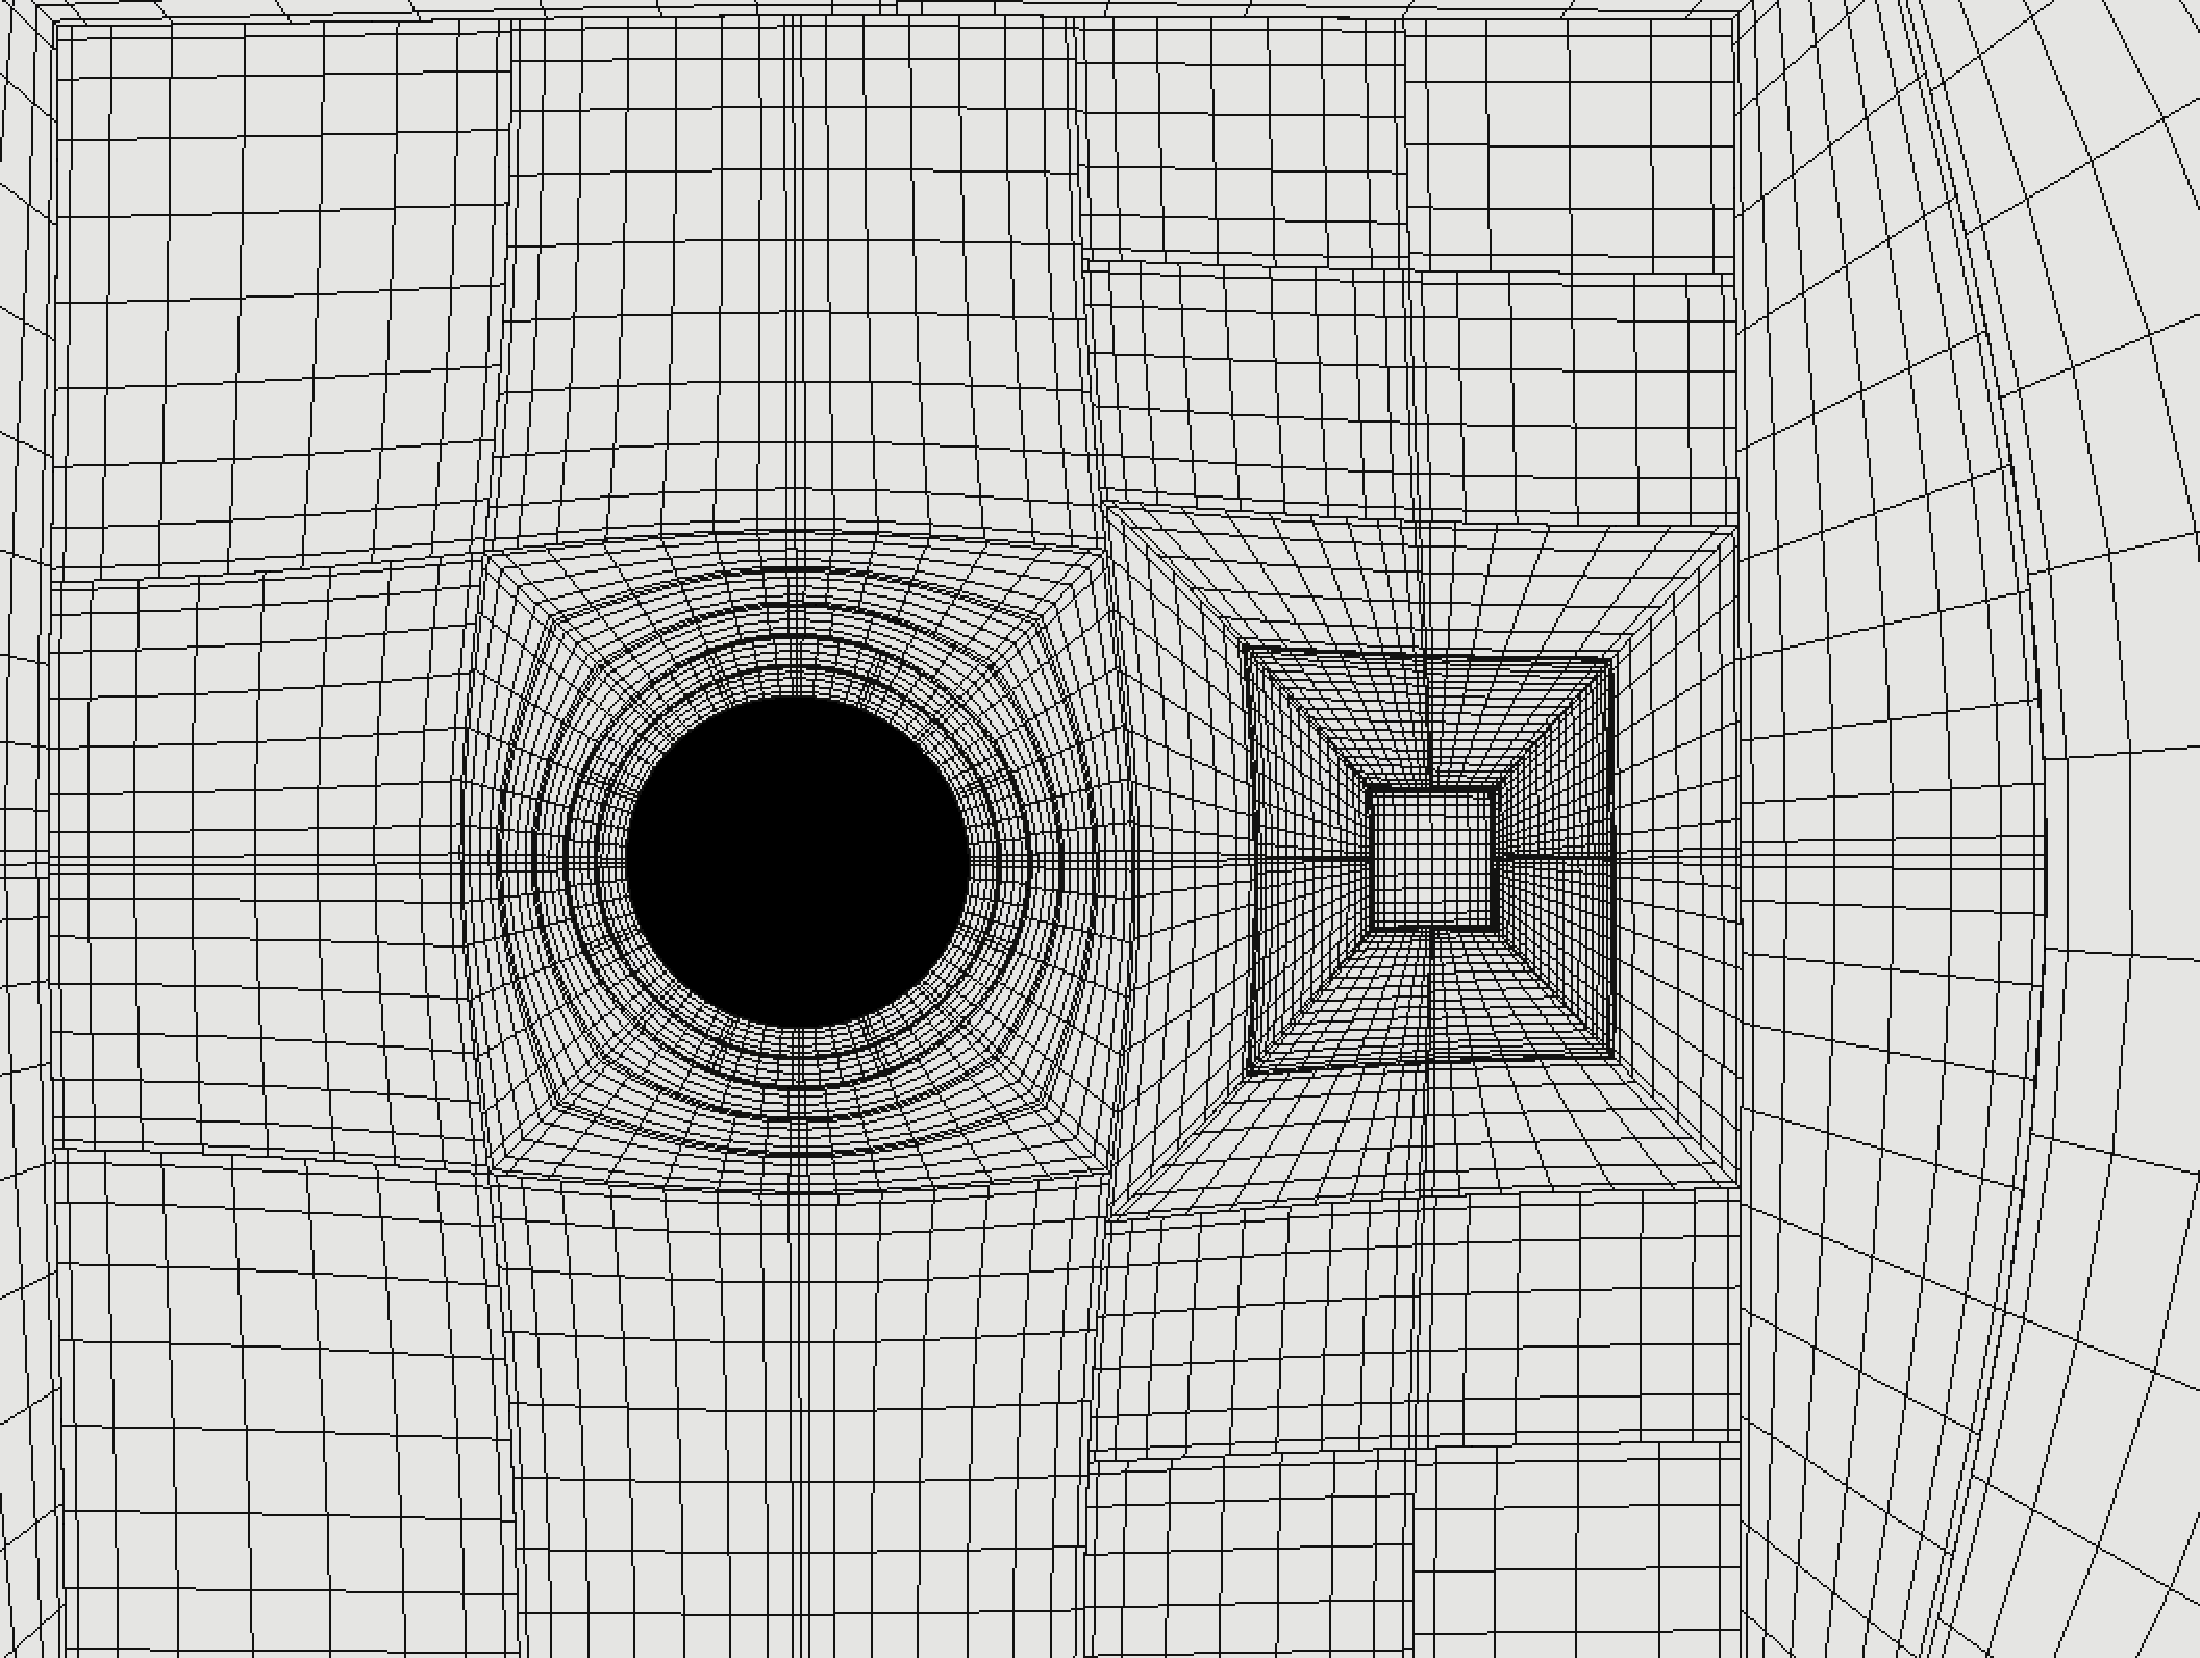
\includegraphics[width=1.0\linewidth]{images/M12_FSU21-pseudospectral-grid}
	\caption[Equatorial slice of the pseudospectral grid]{Equatorial slice of the pseudospectral grid in model M12-M7-S9-FSU21 just before the neutron star begins to accrete onto the black hole.}
	\label{fig:pseudospectral-grid}
\end{figure}

We use pseudospectral methods to evolve the generalized harmonic system, choosing an appropriate set of basis functions for each subdomain configuration.
For example, geometries with an $I1$ (cubes) topology expands solutions in terms of Chebyshev polynomials, spheres S2 use spherical harmonics.
The number of collocation points per subdomains is allowed to grow or shrink in order to maintain a specified truncation error in the elliptic solver.
In addition, subdomains may be split or merged depending on the growth of the collocation points to help maintain load balancing.
In our runs, we only enable this feature of spectral AMR (domain creation) on select runs (i.e., for ADM neutron star masses $M_\textrm{NS} = 1.4 M_\odot$) during peak disruption as the number of collocation points on the distorted cubes outside the excision zone were rapidly growing.
Note that subdividing the subdomains with too many points helps with load balancing and thus simulation speed, but does not affect the accuracy of the simulation speed.
Ideally, we would have just left this feature on and disabled active domain creation once the post-merger remnant has formed.


\section{FD Grid}
\label{sec:fd-grid}

We assume the neutron star matter to be an ideal fluid (see, e.g.~\cite{Duez2005}).  The stress energy tensor is given by
\begin{eqnarray}
T^{\mu \nu} &=& \rho_0 h u^\mu u^\nu + P g^{\mu \nu}.
\label{e:StressEnergyTensor}
\end{eqnarray}
Here, $P$ is the pressure, $g^{\mu \nu}$ the spacetime metric inverse, and $h$ is the specific enthalpy (expressed in terms of the specific internal energy $\epsilon$) given by $h \equiv 1 + \epsilon + P/{\rho c^2}$.
Note that there are two distinct densities used here: the rest mass density, $\rho_0$, and the total energy density, $\rho = \rho_0 + u$ which includes the internal energy, $u = \rho_0 \epsilon$.

The equations governing the fluid in general relativistic hydrodynamics are
\begin{eqnarray}
\nabla_\mu \left( \rho_0 u^\mu \right) &=& 0, \label{e:ConsOfMass} \\
\nabla_\mu T^{\mu \nu} &=& 0, \label{e:ConsOfEnergyMomentum}
\end{eqnarray}
where $u^\mu$ is the four-velocity.  Equation \ref{e:ConsOfMass} represents the conservation of mass of the fluid, while Equation \ref{e:ConsOfEnergyMomentum} represents the conservation of energy-momentum, giving us a total of five simultaneous equations to evolve. 

Following Section \ref{sec:gr-grid}, it is imperative that we evolve the general relativistic hydrodynamic equations in a conservative form.  We thus evolve the ``conservative'' variables
\begin{align}
\label{e:RhoStar}
\rho_*	&\equiv& -\sqrt{g} n_\mu u^\mu \rho_0 
		&=& \sqrt{g} W \rho_0, \\
\label{e:Tau}
\tau 	&\equiv& \sqrt{g} n_\mu n_\nu T^{\mu\nu} - \rho_* 
		&=& \rho_* \left(u^t h - 1\right) - \sqrt{g} P, \\
\label{e:Sflux}
S_i  	&\equiv& -\sqrt{g} n_\mu T^\mu_i 
		&=& \rho_* h u_i
\end{align}
where we have used the general relativistic Lorentz factor $W \equiv \alpha u^t$, the future directed unit normal to the foliated subspace slices is $n^\mu$, and $g$ is the determinant of the spatial \mbox{metric, $g_{ij}$}.  Here we have a matter term, $\rho_*$, an energy term, $\tau$ and the momenta, $S_i$.  The Lorentz factor is given by the normalization condition $W^2 = 1 + g^{ij} u_i u_j$

The fluid equations \ref{e:ConsOfMass} and \ref{e:ConsOfEnergyMomentum} can then be expressed in conservative form:
\begin{align}
\label{e:ADMConsOfMass}
\partial_t \rho_* + \partial_i \rho_* v^i 
	&= 0, \\
\label{e:ADMConsOfEnergy}
\partial_t \tau + \partial_i \left(\alpha^2 \sqrt{g} T^{0 i} - \rho_*v^i\right) 
	&= -\alpha \sqrt{g} T^{\mu \nu} \nabla_\mu n_\nu, \\
\label{e:ADMConsofMomentum}
\partial_t S_j + \partial_i\left(\alpha \sqrt{g}T^i_{\,\,\,j}\right) 
	&= \frac{1}{2} \alpha \sqrt{g} T^{\mu \nu} \partial_j g_{\mu \nu}
\end{align}
where $v^i$ is the fluid three-velocity.  That is, each of the equations is in conservative form $\partial_t u  + \partial_i F^i = \sigma$, for  fluxes $F$ and  source term $\sigma$.  

In addition to the above evolution equations, we evolve the conservative counterpart of the composition variable $\rho_* Y_e$ using the neutrino leakage scheme described in~\cite{Deaton2013}.
That is, the neutrino radiation field appears only as source terms in the evolution equations.
In terms of the effective energy emission rate $Q_\nu$, neutrino radiation pressure $P_\nu$ and the effective lepton number emission rate $R_\nu$, the additional composition evolution equations are, in a local comoving frame of the fluid, 
\begin{align}
\partial_t T^{00} &= -Q_\nu \\
\partial_t T_{j0} &= - \partial_j P_\nu \\
\partial_t (\rho_* Y_e) &= -R_\nu m_U ,
\end{align}
where $m_U$ is the atomic mass unit.

To evolve the fluid equations \ref{e:ADMConsOfMass} - \ref{e:ADMConsofMomentum}, there are a variety of different FD grid configurations and finite difference reconstructors available to \SpEC.
For our simulations, we use a fifth-order accurate, shock-capturing, weighted essentially non-oscillatory reconstruction scheme, WENO5, to perform interpolation of the conservative variables on the grid points to conservative fluxes on cell faces~\cite{Liu1994200,Jiang1996202}.
An HLLE approximate Riemann solver is used to compute the differences of the cell boundary fluxes~\cite{HLL}.
In Section \ref{sec:communication}, we discuss the time integral used, while in Section \ref{sec:hydro-amr}, we will discuss the geometrical configuration of the finite difference grid.

There are also a number of further physical constraints we must safeguard against.
When evolving the conservative variables ($\rho_*$, $\tau$, $S_i$) in low-density regimes, small numerical errors can lead to very large and nonphysical values for the primitive variables (pressure $P$, temperature $T$, velocities $v_i$).
To fix this, we employ two techniques to enforce restrictions on the variables to help prevent them from feeding nonphysical junk into the evolution equations.

\subsection*{Fix Point Parameters}

Before conversion to primitive variables, we first perform truncation calculations on the conservative quantities.  Noninvertible values of the conservative quantities occur when
\begin{equation}
\frac{S^j S_j}{\rho_*^2} \le \tilde{S}_\textrm{max}^2 \equiv \frac{\tau}{\rho_*}\left(2+\frac{\tau}{\rho_*}\right).
\end{equation}
At each step, we impose the condition that
\begin{equation}
\frac{S^j S_j}{\rho_*^2} \le \alpha \tilde{S}_\textrm{max}^2
\end{equation}
where we set $\alpha = 0.999$ when $\rho_* \ge \rho_\textrm{crit} \equiv  10^{-3} \sqrt{g} \rho_0^\textrm{max}(t)$.  For lower densities, we further enforce that 
\begin{equation}
\alpha = 0.999 - 0.0005 \log_{10}{\frac{\rho_*}{\rho_\textrm{crit}}}.
\end{equation}
After these ``fix points'' constraints are enforced, the fixed conservative quantities are inverted back to primitive variables and cleaned with the ``atmosphere parameters''.

\subsection*{Atmosphere Parameters}

Further fixes are applied after primitive conversion.
First, in regions where the (physical) density $\rho_0 < 10^{-6} \rho_0^\textrm{max}(t)$, with $\rho_0^\textrm{max}(t)$ the maximum rest mass density on the grid at a given time, we set $T=0$ and $u_i=0$.
On the other end, we prevent negative densities by enforcing that $\rho_0 > 10^{-11} \rho_0^\textrm{max}(t=0)$ at all points.
We also note that the reference density $\rho_0^\textrm{max}(t)$ is also ``smoothed'' so that the occasional high density spike cannot zap the rest of the points on the grid.
Density thresholds are also multiplied by a so-called ``atmosphere multiplier'', which contains a spherical Gaussian around the black hole:
\begin{equation}
\xi_1 \equiv {e^{- \left(2 \frac{ r_\textrm{dist}[i] - r_\textrm{exc}}{r_\textrm{exc}}\right)}}^2 ,
\end{equation}
where $r_\textrm{exc}$ is the excision radius around the black hole and $ r_\textrm{dist}[i]$ is the distance of grid point $i$ from the black hole.
Before the merger, the density thresholds are multiplied by $\xi_\textrm{ins} = 1 + 100 \xi_1$.  But during the merger, we instead multiply by $\xi_\textrm{dis}  = 10^{-3} + 100 \xi_1 + \xi_2$, where $\xi_2$ is the damping parameter defined as
\begin{eqnarray}
\xi_2 = 4 \left( \frac{r_\textrm{exc} + r_\textrm{NS}}
{ r_\textrm{dist}[i] + r_\textrm{exc} + r_\textrm{NS}}\right)^2 , 
\end{eqnarray}
and $ r_\textrm{NS}$ the initial radius of the star.
Heuristically, the Gaussian component $\xi_1$ enforces higher cutoff values in the vicinity of the black hole and lower cutoffs far away.
The damping component $\xi_2$ is engaged only during the merger to increase the density threshold between the intertial matter and the apparent horizon.
We do not allow a pure vacuum in our code, as velocity would not be defined for zero-densities.  Therefore, an absolute density floor is set to $\rho_0 >  \rho_\textrm{floor} = 10^{-14} \rho_0(t)_\textrm{max}$.  

In general, there are three ways to control the temperature in our code, either via: enthalpy constraints, controlling the polytopic constant, $K = P/{\rho^{\Gamma}}$ or through the temperature directly.
In our simulations, it is more straightforward to restrict the temperature via the latter, since our equation of state is directly dependent on the temperature.
In low density regions where $\rho_0 \le 10^{-11} \rho_0^\textrm{max}(t)$, we do not allow the temperature to exceed $T_\textrm{max} < 100\,\textrm{MeV}$.
We also applied $T < T_\textrm{max}$ globally, i.e. even in low density regions since this is the upper limit of the highest temperature bin in the our equation of state tables.  
Conversely, while the equation of state tables may go down to $0.01 \textrm{MeV}$, we set the temperature minimum to $T_\textrm{min} = 0.5 \textrm{MeV}$ in the low density $\rho_0 \le 10^{-11} \rho_0^\textrm{max}(t)$ regions as the $T < T_\textrm{min}$ bins are typically inaccurate in the tables.

Errors in the density profile or non-smooth bins in the equation of state can lead to errant temperature spikes.
On those grid points, and if the density is below the threshold, we zap temperature spikes by replacing the temperature with averaged values from its neighboring points.
More commonly, these temperature deltas are much more attributable to numerical error.
We impose a maximum on the Lorentz factor $W = \alpha u^t$ by constraining $u \equiv \sqrt{g^{ij} u_i u_j} < 1000$ in low density regions.


\section{Time-steps and communicating source terms}
\label{sec:communication}

Both systems of equations are evolved jointly and coupled through the interpolation between the metric and fluid variables. 
For instance, after each time-step, both systems compute the time integral with a third-order Runge-Kutta solver.
The source terms are then communicated between the two grids after each time step:

(1) The fix-point corrected evolved conservative fluid variables ($\rho_*, \tau, S_i, Y_e$ of Equations \ref{e:RhoStar} - \ref{e:Sflux}) are transformed back to primitive variables ($\rho_0, h, W, P, u_i$) on the fluid grid.  After atmosphere-paramater corrections are applied, the primitives are then communicated to the pseudospectral grid, where the stress energy tensor $T^{\mu\nu}$ is computed (see Equation \ref{e:StressEnergyTensor}).  The FD $\rightarrow$ GR interpolation uses a third-order shock-capturing WENO3 interpolator. 

(2) The evolved metric quantities from the pseudospectral grid ($g_{ij}, \partial_i g_{jk}, \beta^i, \partial_i \beta^j, \alpha, \partial_i \alpha,  K_{ij}$) are likewise communicated to the finite volume grid to provide the metric quantities in and compute the source terms on the right hand side of Equations \ref{e:ADMConsOfMass} - \ref{e:ADMConsofMomentum}.  The GR grid is derefined in this step (only every third point on the pseudospectral grid has non-zero coefficients for the basis functions) for efficiency.  The GR $\rightarrow$ FD communication uses a polynomial interpolator with fourth-order accuracy.
In the final step of this communication, we convert the primitives back to conservative form.

The fluid grid, divided into many subdomains, is deployed for use in massive parallel computing environments where each subdomain (or an integral number of them) can be assigned to a specific processor. 
At subdomain boundaries, most finite difference/finite volume schemes lose design order accuracy when approaching the final few boundary points since the stencil loses the requisite number of cell centers (or faces) to do reconstruction.
In our code, we use overlapping ``ghost zones'' at subdomain interfaces, in that we add three extra points in positive inertial directions and two in the negative.
The terminal and penultimate points at interfaces have data that is  replaced---since they aren't covered by a full stencil---by points that do in order to interpolate accurate derivatives.
Other finite volume schemes like ESWENO (with boundary closures) have a very robust stencil that can guarantee third order accuracy without the need of ghost zones.  
Continuous meshing schemes like the Discontinuous-Galerkin method are also being explored within \SpEC.



\section{Hydro-AMR Algorithm}
\label{sec:hydro-amr}

Prior FD-grid structures in \SpEC for evolving black hole-neutron star systems involved using a Cartesian, cubic ``unigrid'', where the grid consisted of a number of equally sized subdomains defined to extend to a specified outer boundary.  
Unigrids, however, can only evolve the large tail region well and the accreting tail poorly, or they can evolve the interior protodisk well while limited to evolving the matter outflow.  
You cannot do both.  
The accretion disk spans an areal radius $\sym 50 \textrm{km}$.  
In linear space, the width of the tail for high spin black holes can be as thin as $\sym 5 \textrm{km}$ across.  
To capture the interesting properties of the ejecta, the tail material must be captured well out of the frame at length scales comparable to the excision radius, to the tune of $\sym 1000 \textrm{km}$.

A first try at improving the cubic grid structure was a test implementation of ``fixed'' mesh refinement.
The subdomain cubes could be expanded every $2\,N_\textrm{ext}\,dx_i$ from a central point, where $N^i_\textrm{ext}$ is the number of points along spatial dimension $x_i$.
At each level of refinement the grid spacing doubles.
Note that in our implementation, each subdomain has an equal number of points regardless of refinement level.
Therefore, when we double the \textit{size} of a subdomain, we are \textit{halving} its resolution.

Although this method provides the proper resolution to evolve both the longer tail material and the resulting accretion disk, only $\left(10 - 20\right) \%$ of the subdomains during peak disruption are evolving matter.  
To improve on this further, we've introduced in~\cite{FoucartDD2:2017} a new implementation of an adaptive mesh refinement (AMR) algorithm that can turn  fluid subdomains off and on.
In general, we use $7$ levels of refinement, where each each subdomain has $300 \times 300 \times 200$ points in each Cartesian direction.
Each refinement level is then divided into $12 \times 12 \times 8$ subdomains.
The innermost finest level can evolve any of its subdomains so long as they are not completely enveloped within the excision region around the black hole.
For each of the outer six levels, the central $6 \times 6 \times 4$ are never evolved since they overlap the inner level.

To implement an algorithm for \textit{how} a subdomain is turned on, we check that if any cell within $6$ grid spacings (safely away from the ghost zones) from the outer boundary, the fluid density satisfies 
\begin{equation}
\rho > \rho_\textrm{FMR} 
	\equiv 3 \times 10^{10}\left[0.001 
	+ \left( \frac{2 r_\textrm{exc}}{r+r_\textrm{exc}} \right)
	\right] \textrm{g}\,\textrm{cm}^{-3}
\end{equation}
where $r_\textrm{exc}$ is the excision radius and $r$ the coordinate distance from the black hole center, in the coordinates of the spectral grid.
Conversely, if the fluid density is $\rho < \rho_\textrm{FMR} / 2$ for every cell within $6$ grid points from the outer boundary.
We perform these two checks every $20$ time steps.

The numerous limitations of our Hydro-AMR algorithm are indeed an open place for improvement.  For instance, the size of the subdomains is still very much fixed, and must be manually adjusted when material is under resolved (or over resolved).  An improvement here would be to develop a criterion to adjust the subdomain block size anywhere on the grid as other fluid codes do~\cite{YamamotoShibata2008} (as does the pseudospectral method used in the evolution of Einstein's equations in our code), regardless of the evolution center.  

\section{Phases of the evolution}
\label{sec:epochs}

\subsection{Initial Data} As described in Chapter \ref{chap:chapter-2}, we construct the neutron star using the available Equation of State tables which contain a multidimensional relationship of baryonic rest mass density, $\rho_0$, temperature, $T$, and composition, $Y_e$.  In our study, our neutron stars have a ADM masses of $1.2 M_\odot$ and $1.4 M_\odot$ that span the expected range of observed neutron star masses in binary orbits~\cite{Ozel2012}.  The star's initial temperature is cold, set at $0.01\,\textrm{MeV}$.  We choose the parameters of the black hole to yield a result that is highly disruptive to the fluid matter by prescribing a high, prograde-aligned spin of $a_* \equiv J_\textrm{BH}/M_\textrm{BH}^2 = 0.9$ and a Christodoulou mass of $7 M_\odot$, for each system, to be more conducive to tidal disruption and less likely for the star to directly plunge into the black hole.
In general, an orbitally aligned highly spinning black hole brings the innermost stable circular orbit (ISCO) closer to the horizon.
The neutron star will maximally disrupt the closer the ISCO is to the black hole, since the  neutron star will disrupt deeper into the potential well.

\subsection{Inspiral}
The initial separation between the two objects is chosen so that the system may quasicircularly orbit $4-5$ times (providing $\sym 8-10$ full gravitational wavelengths).  
We evolved the fluid grid in the upper-half of the orbital plane assuming equatorial symmetry to the lower-half matter.  While nonconservative matter fluxes across the equator \textit{are} an issue during the plunge, we can still safely utilize equatorial symmetry during the inspiral.  
In addition, we used a cubic unigrid for this epoch since the technology from Section \ref{sec:hydro-amr} wasn't yet available.
An additional (although, in the large scheme, minor) benefit was that the number of requested processors could be halved.  
The box-size of the fluid grid was roughly set to $2 R_\textrm{NS}$.  
The termination criteria for the inspiral in all simulations occurred when the binary separation dropped below a specified expansion factor, which is based on the neutron star's Hill radius.
During this phase, we use a frozen harmonic gauge where the components of $H_a$ are all set to zero.  
	
\subsection{Plunge}  
The transition from inspiral to the ``plunge'' epoch of the merger, i.e. when tidal disruption starts, accelerating the accretion rate onto the black hole, required several steps.  First, the evolved upper-half fluid variables on the finite-difference grid must be reflected onto the lower-half, using a domain reflector tool in \SpEC.  Second, the new cubic Hydro-AMR domain needs to be constructed from the unigrid domain used during inspiral.

With previous BHNS evolutions in \SpEC, including the inspiral portion of the simulations in this work, the fluid grid was evolved in separate, comoving ``grid'' coordinates, while the GR grid was evolved in ``spectral'' coordinates.  An accompanying interpolation was needed to transform between the two coordinate systems after each time step.
In the new AMR framework, implemented from the plunge phase onward in our simulations, both grids use the same coordinate (spectral) system, so no map between them is necessary. 

We allow the Hydro-AMR grid to be able to expand up to four levels of refinement with a total span of $\sym(1200 \times 600 \times 600)\, \textrm{km}$, although no more than two levels were used (span a factor of four smaller) in all eight of our simulations.
However, this procedure can be tricky. 
The star is still mostly spherical, in the frame comoving with the grid, but will quickly tidally deform due to the highly curved black hole spacetime.
The new fluid grid must \textit{a priori} be constructed to allow the creation of future subdomains according to a rough approximation of how the star will distort (we treat previous simulations as a rough prediction), given the symmetries of the system.
To accomplish this, we determine the center of the new FD grid visually and envelop the two objects in a rectangular box with the finest level of refinement.  
Since most of the disruption points radially toward the black hole, the corotating system allows us to follow the matter with a single prolonged axis defined by the line between the neutron star and the black hole, extending from one binary object to the other.
Because the inspiral grid contained only the neutron star, most of the available subdomains ($\sym 70\%$) will overlap the vacuum.  
Therefore, to generate the new domain, we use our convention that starting from the corner subdomain in the negative Cartesian octant, subdomains are annotated integrally and stride along the positive direction to the outer, positive-sided boundary.
At this stage, the star is still mostly spherical, so generating the subdomains in the initial cubic configuration of the star is fairly straightforward.

We also modify the gauge function $H_a$ to a damped harmonic gauge discussed in~\cite{Szilagyi:2014fna}.  To smoothly transition to the new gauge from the frozen harmonic gauge used during inspiral, we roll on the damped harmonic gauge by setting
\begin{equation}
\partial_t H_a = f_\textrm{d}(t) (\partial_t H_a)_\textrm{damp} + (1 - f_\textrm{d}(t)) (\partial_t H_a)_\textrm{frozen}
\end{equation}
where 
\begin{equation}
f_\textrm{d}(t) = 1 - e^{ \left(\frac{t-t_\textrm{d}}{w_\textrm{d}} \right)^4 }
\end{equation}
and the width parameter $w_\textrm{d}$ is a timescale set to $20 M$ after which the damped harmonic gauge is fully turned on.  In our simulations (total system mass $M \sym 8 M_\odot$), the DH gauge takes over in just under a millisecond from the onset of accretion.

This epoch lasts between $1 - 2$ orbits.

\subsection{Post disruption}

Once half of the neutron star mass has been accreted onto the black hole, we begin the final stage of the merger.  
Since we expect an axisymmetric accretion disk to form, there is no longer a need use a rotational coordinate system.
In addition, a sizable amount of the mass in the outer tail becomes unbound and will be ejected from the system.  
The final post-merger remnant will axisymmetrize around the black hole.
However, we must again determine the appropriate grid for the new epoch.

To avoid interpolating the primitive variables on restart, we center the grid an integral number of grid spaces from the center of the black hole, with the finest level capturing the infalling material where shocks are most likely to occur.  
We bump the number of allowed levels from $4$ to $7$ to capture the outflow, with a total span of $\sym(4800 \times 4800 \times 3200) \textrm{km}$, although no more than $6$ levels were used in all eight of our simulations.
Note that we symmetrized the boundaries of the $x$ and $y$ axes, whereas in plunge, $y$ and $z$ were symmetrized (we lose the coratating frame so the matter will secularly distort in the $xy$-plane).    

After the leading edge of the infalling tail within the finest level begins to fully surround the horizon on the equator, we reduce the resolution of the finest grid to that of the next outer grid. 
In this stage, the fluid around the apparent horizon begins to form a protodisk.
Once this protodisk (roughly) begins to axisymmetrize, we reduce the resolution of the finest level a second and final time, resulting in five levels of refinement before the matter leaves the grid.

As for the post-merger remnant and fallback material, no further adjustments to the grid are performed.









